\documentclass[letta4 paper]{article}
% Set target color model to RGB
\usepackage[inner=2.0cm,outer=2.0cm,top=2.5cm,bottom=2.5cm]{geometry}
\usepackage{setspace}
\usepackage[rgb]{xcolor}
\usepackage{verbatim}
\usepackage{subcaption}
\usepackage{amsgen,amsmath,amstext,amsbsy,amsopn,tikz,amssymb,tkz-linknodes}
\usepackage{fancyhdr}
\usepackage[colorlinks=true, urlcolor=blue,  linkcolor=blue, citecolor=blue]{hyperref}
\usepackage[colorinlistoftodos]{todonotes}
\usepackage{rotating}
\usepackage{listings}
%\usetikzlibrary{through,backgrounds}
\hypersetup{%
pdfauthor={Siddharth Singh},%
pdftitle={Homework},%
pdfkeywords={Tikz,latex,bootstrap,uncertaintes},%
pdfcreator={PDFLaTeX},%
pdfproducer={PDFLaTeX},%
}
%\usetikzlibrary{shadows}
% \usepackage[francais]{babel}
\usepackage{booktabs}
\newcommand{\ra}[1]{\renewcommand{\arraystretch}{#1}}

\newtheorem{thm}{Theorem}[section]
\newtheorem{prop}[thm]{Proposition}
\newtheorem{lem}[thm]{Lemma}
\newtheorem{cor}[thm]{Corollary}
\newtheorem{defn}[thm]{Definition}
\newtheorem{rem}[thm]{Remark}
\numberwithin{equation}{section}

\newcommand{\homework}[6]{
   \pagestyle{myheadings}
   \thispagestyle{plain}
   \newpage
   \setcounter{page}{1}
   \noindent
   \begin{center}
   \framebox{
      \vbox{\vspace{2mm}
    \hbox to 6.28in { {\bf ESE-680 - Autonomous Racing \hfill {\small (#2)}} }
       \vspace{6mm}
       \hbox to 6.28in { {\Large \hfill #1  \hfill} }
       \vspace{6mm}
       \hbox to 6.28in { {\it Instructor: {\rm #3} \hfill Name: {\rm #5}, PennID: {\rm #6}} }
       %\hbox to 6.28in { {\it TA: #4  \hfill #6}}
      \vspace{2mm}}
   }
   \end{center}
   \markboth{#5 -- #1}{#5 -- #1}
   \vspace*{4mm}
}

\newcommand{\problem}[2]{~\\\fbox{\textbf{Problem #1}}\hfill (#2 points)\newline\newline}
\newcommand{\subproblem}[1]{~\newline\textbf{(#1)}}
\newcommand{\D}{\mathcal{D}}
\newcommand{\Hy}{\mathcal{H}}
\newcommand{\VS}{\textrm{VS}}
\newcommand{\solution}{~\newline\textbf{\textit{(Solution)}} }

\newcommand{\bbF}{\mathbb{F}}
\newcommand{\bbX}{\mathbb{X}}
\newcommand{\bI}{\mathbf{I}}
\newcommand{\bX}{\mathbf{X}}
\newcommand{\bY}{\mathbf{Y}}
\newcommand{\bepsilon}{\boldsymbol{\epsilon}}
\newcommand{\balpha}{\boldsymbol{\alpha}}
\newcommand{\bbeta}{\boldsymbol{\beta}}
\newcommand{\0}{\mathbf{0}}


\begin{document}
\homework{Perception and Vision}{Due: 11/23/19}{Rahul Mangharam}{}{Student name(s)}{NetId(s)}

\noindent\textbf{Note:} This is a \textbf{GROUP} assignment.

\section{Overview}
Most racing series feature multiple vehicles competing simultaneously on a single track. As such, safely overtaking and navigating in the presence of other vehicles is paramount to performing well. Since the strategy and decisions of of other vehicles cannot be known ahead of time and may, in fact, be stochastic it is necessary for your car to react to new constraints imposed by other vehicles online.
Thus, the goal of this lab is to track and predict the pose of an opponent vehicle (see Fig. \ref{fig:overview})
%We would be using implemented packages and machine learning algorithms to create a decision making pipeline which will help your vehicle perform maneuvers such as overtaking and high speed turning.\\
%As a thought, if you could predict with some amount of probability the path that the vehicle in the front is about to take, it will increase your chances of safe overtaking by a significant amount.\\
%By the end of this lab, you would be able to do things like these: 
\begin{figure}[h!b]
  \centering
    % replace sample_figure.png with your image file in this folder
    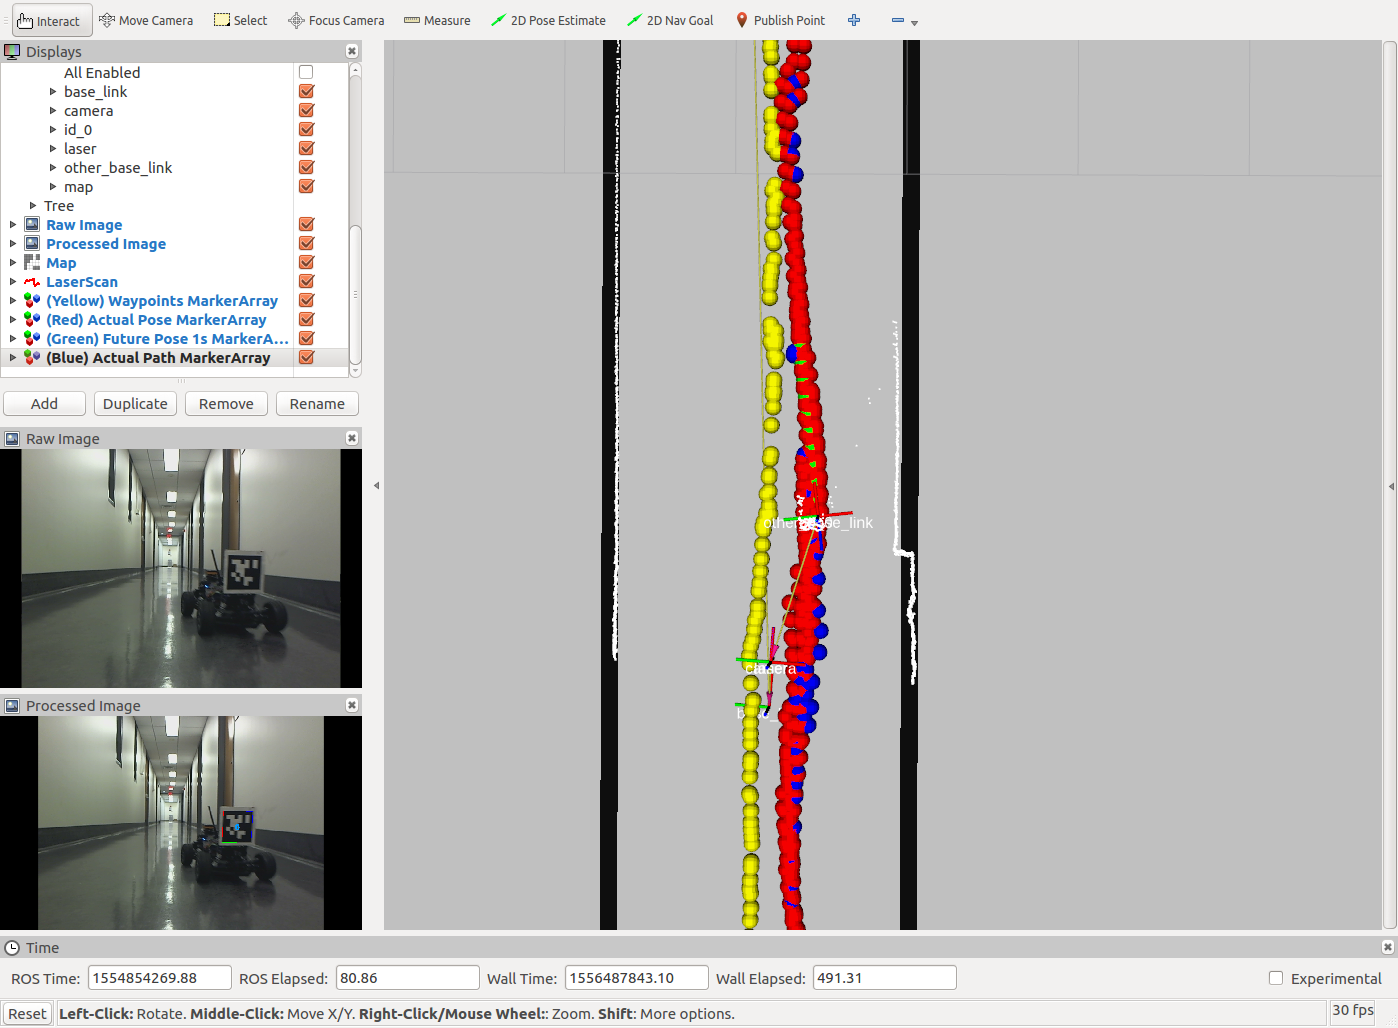
\includegraphics[width=\textwidth]{actual-versus-predicted-path-13.png}
   \caption{Tracking and predicting the pose of an opponent}
   \label{fig:overview}
\end{figure}

\noindent\textbf{Course Policy}: Read all the instructions below carefully before you start working on the assignment, and before you make a submission. This is a group assignment to be completed by each team independently. All sources of material must be cited. The University Academic Code of Conduct will be strictly enforced.
\subsection{Goals and Learning outcomes}
\begin{itemize}
    \item \textbf{Vision and Perception}
    \begin{itemize}
        \item \textit{Camera model and parameters:}
        You should be able to understand how the real camera model and the pin hole camera model are related and what assumptions are made while going from the former to the latter.
        \item \textit{Transformations:}
        You should be able to understand 3 dimensional transformations and know the representations of transformations. 
        \item \textit{Single View Geometry:}
        You should be able to understand and work with single view geometry and how world coordinate frame points translate to camera coordinate frame points. 
        \item \textit{Homography:}
        You should be able to work with homography and how it can be used to calculate pose of the camera given the world coordinate correspondances. 
    \end{itemize}{}
    
    \item \textbf{Programming skills }
    \begin{itemize}
        \item Working with images on ROS
        \item Transformations using tf and implementation of AprilTags ( and similar) librarie(s). \item Implementing nodelets in ROS and their advantages. 
    \end{itemize}{}
    
    % \item Deep learning Vision
    % \begin{itemize}
    %     \item Learn the use of Pre-trained model YOLO (You only look once) 
    %     \item Learn how detection can be used to speed up the vision pipe line. 
    % \end{itemize}{}
\end{itemize}
\\
% \textbf{The Lab is divided into the following broad take away:} \\
% 1. Conceptual exercises : Problem 1 \\
% 2. Implementation and setup of Camera and Vision modules: Problem 2: Part a and b \\
% 3. Implementing algorithm of Vehicle tracking and prediction: Problem 2: Part c \\
% 4. Core Programming : Problem 2, Part d\\
% 5. Vision with Deep Learning : Problem 2 part e \\
% 6. Testing and results : Problem 2 , Part f \\
% \\
% \textbf{From the lab exercises, parts a and b are supposed to be in-lab exercises so that you can have sufficient time to work on the algorithms and the various other parts of the lab. }
% \clearpage

% \problem{1:Written Problems}{}
% \subproblem{a: Homography} 
% \\Write your solution here (or include the solution image file)

% \subproblem{b: Perspective 3 Point formulation} 
% \\Write your solution here(or include the solution image file)

% Comment: In the objective, we wrote ``Practice writing proofs'' but this is rather simple and not very rigorous?

%\newpage
% \problem{Lab Assignment}{}
\clearpage
% \section{Camera Setup and Calibration}
% \begin{figure}[h!b]
%   \centering
%     % replace sample_figure.png with your image file in this folder
%     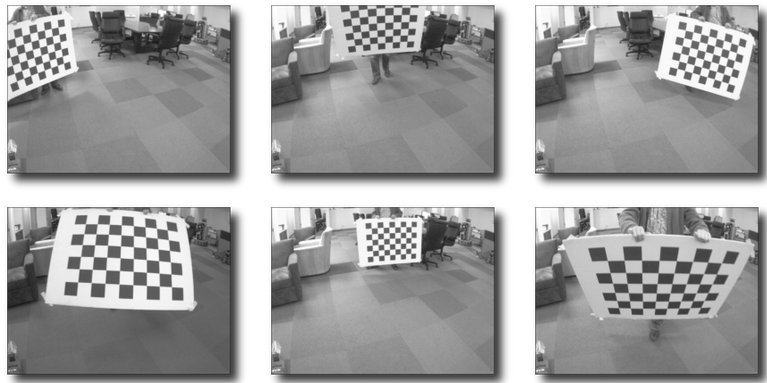
\includegraphics[width=0.5\textwidth]{calibration.png}
%   \caption{Calibrating the camera}
%   \label{fig:calibration}
% \end{figure}

% \subsection{Install required packages}
% Note that for this lab we will work with ROSBAG files instead of hardware. Recall that many of the techniques we have discussed in lecture require the camera intrinsics. Thus,
% we must perform camera calibration in order to obtain the parameters of the intrinsic matrix. In order to standardize the task we have created a ROSBAG which contains images of a a calibration checkerboard in multiple poses relative to the cameras frame (see Fig.~\ref{fig:calibration}). The purpose of this portion of the lab is to gain familiarity with the tools available in the ROS ecosystem for camera calibration. For the final race you may choose from a variety of camera hardware and will need to use these tools. \\

% First you will need to obtain the ROSBAG which will be used for calibration from: \textbf{ADD a link here}. When integrating new hardware for the final race this is a useful command to check that images are being published.
% Once you have the data try visualizing the image topic using rqt image viewer:
% \begin{lstlisting}[language=bash]
%   $ rosrun rqt_image_view rqt_image_view
% \end{lstlisting}\\

% %Clone the following repository \textbf{ADD a link} which can subscribe to the bag file. \\
% %(\textbf{Note: we are not going to use the camera parameters found through this calibration in the tracking prediction implementation. You will be provided with a camera calibration parameter file for that.})
% %use rqt image viewer to check that the raw image is being published over a topic. 

% % \textbf{2. }Now you know to which topic the images are being published. In the skeleton repository we have already included this topic so you do not have to worry about this there. You will not be subscribing to this topic because serializing and tossing around images over a ROS network is very expensive. Instead, we use nodelets in cpp ROS to makes sure that only pointers ( or addresses) of the image are tossed around. You will implement a nodelet of your own in this lab too. \\

% ROS has many useful tools for working with cameras. The image pipeline package contains a camera calibration utility. 
% Obtain the image pipeline from the following repository:
% \href{https://github.com/ros-perception/image_pipeline.git}{image pipeline}.
% The following commands will be used to setup up, install, and run the camera calibrator:\\
% \begin{lstlisting}[language=bash]
%   $ rosdep install camera_calibration
%   $ rosrun camera_calibration cameracalibrator.py --size <> --square <> image:=<topic name>
%   camera:=<camera name>
% \end{lstlisting}

% \subsection{Perform calibration}
% A GUI will open up showing the images from the camera which has been recorded in the ROSBAG.
% Notice that the checkerboard is moved relative to the camera frame such that:
% \begin{itemize}
%     \item The checkerboard appears in the image to the camera's left, right, top and bottom 
%     \item X bar - left/right in field of view
%     \item Y bar - top/bottom in field of view
%     \item Size bar - toward/away and tilt from the camera 
%     \item checkerboard filling the whole field of view
%     \item checkerboard tilted to the left, right, top and bottom (Skew) 
% \end{itemize}

% Once the calibration tool determines that a sufficient number of samples have been obtained, the calibration button in the GUI will light up and you can press it. You may notice that all the straight edges of the square are now also perfectly straight in the image (because the camera intrinsics and extrinsics have been determined). When working with hardware in the future you may press commit to write the calibration to the camera. For this lab you should save the calibration parameters in a yaml file. For a detailed tutorial and also to know how to do calibration for stereo cameras, see the following link: \href{http://wiki.ros.org/camera_calibration/Tutorials/MonocularCalibration}{Detailed tutorial for Camera Calibration}

% \subsection{Deliverables}
% You should submit the yaml file containing the result of your camera calibration. Note: we supply a separate calibration file for the remaining portions of this lab so as to ensure all submissions are comparable. 

\clearpage
\section{Working with AprilTags}
\subsection{Download the required packages }
You can download the package containing the required repositories from this link. \href{https://drive.google.com/open?id=1yCs7dbwPPBzjbPul1k0SwnOg4jth4hTx}{Link}
\subsection{Obtain camera parameters}
The camera parameters and rviz parameters are present in the config/ folder of the repository.

\subsection{Install apriltag\_ros}
Download the required base repositories from this link \href{https://github.com/AprilRobotics/apriltag}{base April Tags}. There are instructions for setting up the base april tags repository. 
First set up the AprilTag repositories, then You will just have to include the folders in the zip file in you src/ folder and compile your workspace. 

\begin{lstlisting}[language=bash]
  $ catkin_make
\end{lstlisting}


\subsection{Set up vehicle tracker and prediction repository}
Once you have AprilTags setup you have to work on the vehicle\_tracking\_prediction repository. Verify that there are no missing dependancies.If the dependencies are installed correctly there should be no compiler errors.\\
Now you will be able to test the basic functionality of the AprilTags library. First, start playback of the recorded sensor data:
\begin{lstlisting}[language=bash]
  $ rosbag play <bagfile>
\end{lstlisting}
Then launch the AprilTag detector:
\begin{lstlisting}[language=bash]
  $ roslaunch vehicle_tracker_prediction_skeleton detect_apriltags.launch
\end{lstlisting}

\begin{figure}
  \centering
    % replace sample_figure.png with your image file in this folder
    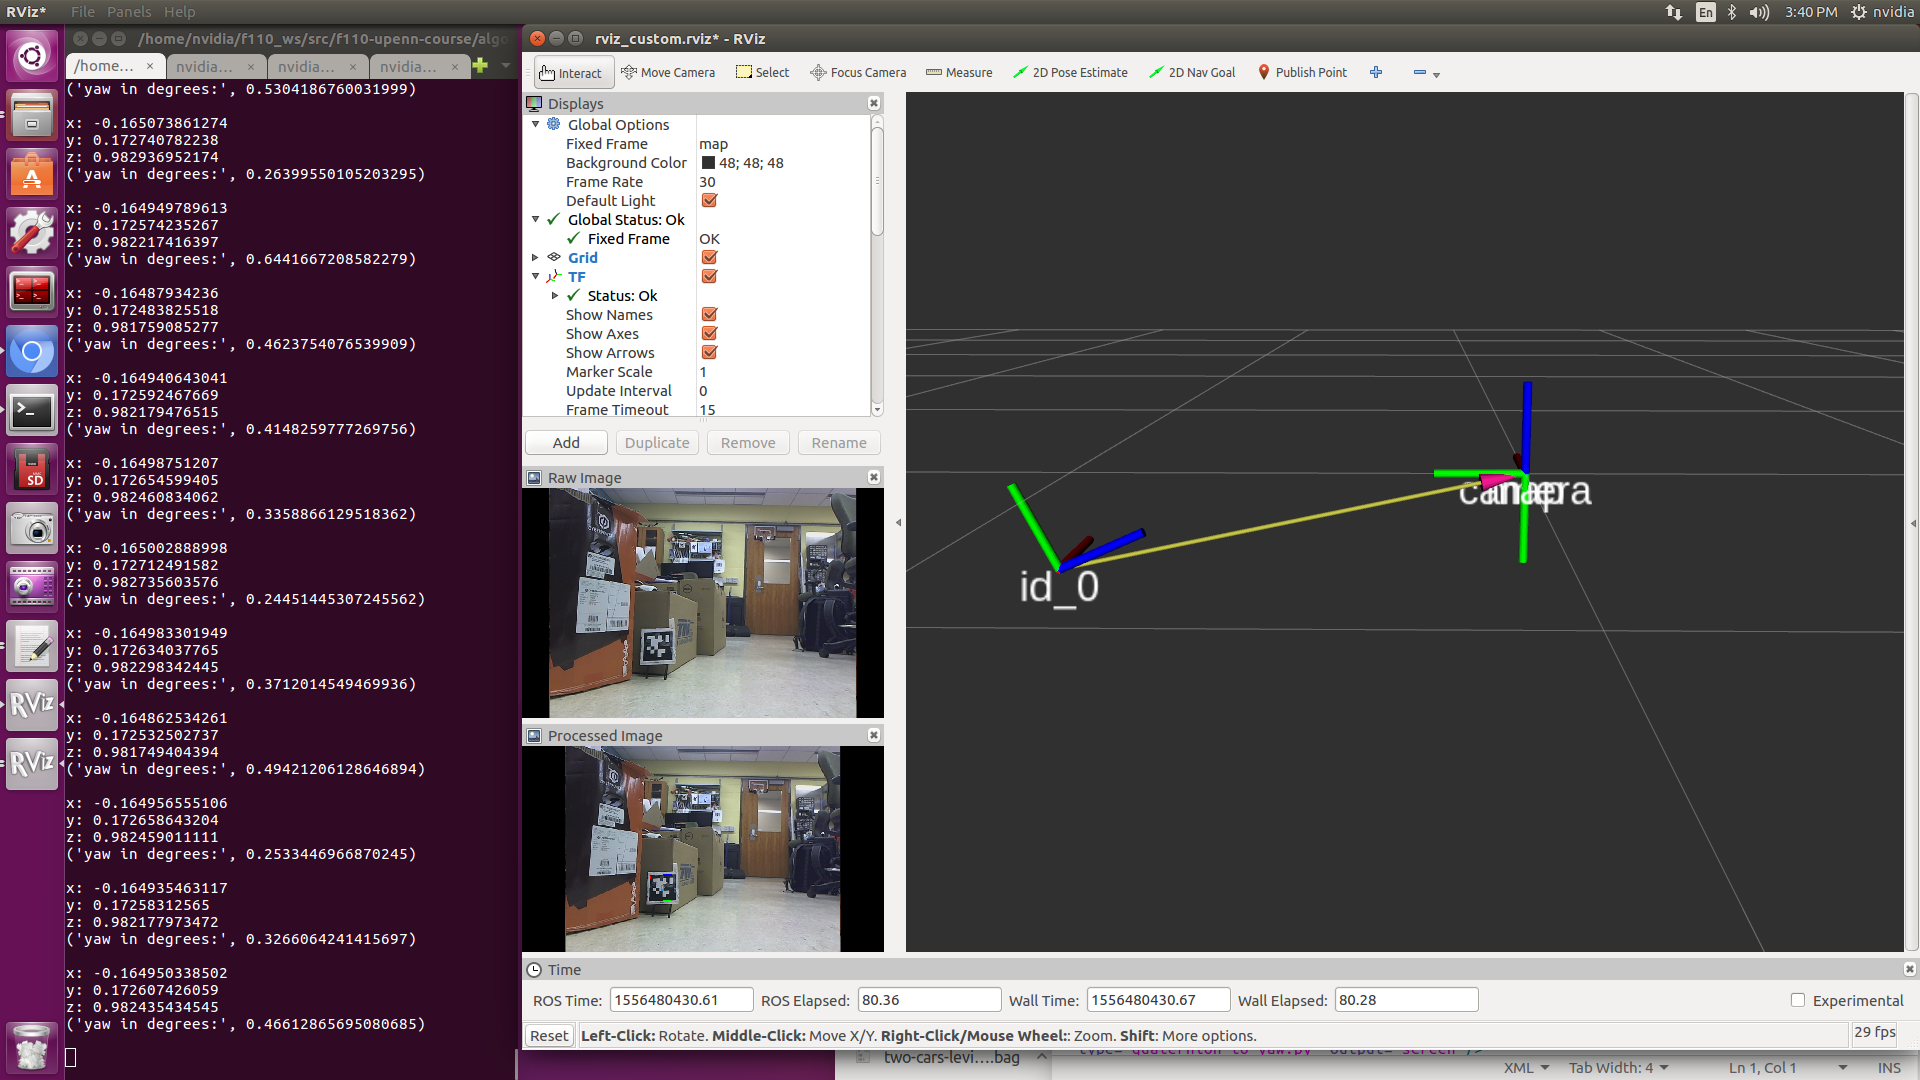
\includegraphics[width=0.5\textwidth]{detect-apriltag-launch.png}
   \caption{Detecting April Tags over Rviz}
\end{figure}

The next step is to modify the following files in the repository

\begin{lstlisting}[language=bash]
  1. Vehicle_Track.cpp
\end{lstlisting}
The following tasks need to be performed by the pose predictor node: 
\begin{itemize}
    \item It should subscribe to /tag\_detections topic with AprilTagsArray message type.
    \item It should implement the weighted prediction algorithm described in lecture. 
    \item You should tune the weighted prediction hyperparameters.
    \item It should publish the poses to a topic called /pose\_predictions which will have a markerarray message type. 
\end{itemize}{}

\subsection{Deliverables}
You should submit the updated vehicle tracker package and clear instructions on how to run your code including any additional dependencies or libraries (e.g. Pure Pursuit implementation).

\clearpage
\section{Convert Nodes to Nodelets}
Using nodelets is a standard practice when it comes to working with images in ROS. Transporting image messages over the standard TCP protocol for pub/sub in ROS creates significant delays. Instead of creating copies of images and passing the data around, nodelets creates shared memory between nodes and pass the pointer to the image in memory instead under a nodelet manager.
The apriltag\_ros wrapper we provided does not run on nodelets, and is not fast enough to provide a robust detection framework. You'll need to convert the bare apriltag\_ros package to run on nodelets.
\textbf{Warning:} Please do not copy any existing code that you can find on the internet to convert to nodelets. We will know if you copied from existing repositories online.\\
% \href{https://github.com/AprilRobotics/apriltag_ros/tree/30629ea495950d961fb093849d021ab811737736}{Bare April Tags Repository}\\
 
 \noindent\textit{References: }\\
 \href{http://wiki.ros.org/nodelet}{ROS wiki}\\
 \href{http://tayyabnaseer.blogspot.com/2013/04/porting-nodes-to-nodelets-in-ros.html}{Blog on porting nodes to nodelets}\\
 \href{https://github.com/cryborg21/sample_nodelet/tree/master/src}{Example nodelet}\\
 \href{https://www.clearpathrobotics.com/assets/guides/ros/Nodelet\%20Everything.html}{Clearpath robotics tutorial}\\

Here are a few steps and tips that you can take to get started.
\begin{itemize}
    
% \item Go through the \texttt{CMakeLists.txt} of both the AprilTag Repository ( the one with the nodelet and one without the nodelet). Notice that the bare repository also has dependency on AprilTags2 while the one with nodelets does not. Why do you think is that? Will that also change your implementation of the nodelets?

\item Everything you need to care about is in the ROS package inside the folder apriltags2\_ros
 
 \item Since we are only using the continuous\_detector node you can only convert this node into a nodelet. \item First, edit the continous\_detector.h file. You will have to make a shared pointer object for the TagDetector Object and also a shared pointed object image\_transoirt object. 
\item  You will have to add the nodelet spec will ifications in the main function in the apriltags2\_ros\_continous\_node.cpp file. 
\item In continuous\_node.cpp you will have explort the pluginlib class list macros and specify the class to be exported. You will have to make the oninit() function and initialize the nodehandles, tag detector objects, image transport objects, etc. inside it. You can now leave the constructor empty. Ypu might have to make some changes in the image callback function too. 
\item in the cmake list you will have to take care of the dependencies such as pluginlib and nodelet. Make sure your executable and libraries are defined correctly for the continuous node detector
\item You will create a new .xml file called the nodelet\_plugins.xml file and specify the library path and the class path. 
\item You will change the package.xml file to specify the dependencies of nodelets and pluginlib and also export the nodelet\_plugins.xml file. This will be loaded during runtime. 
% \item Look into the XML Files and the cmake lists. You will have to make changes to that.
 
% \item Notice which node is being launched by the Vehicle Tracker? Try to nodelet only that node. Please take care, that node might depend on other node too ( might not? ) just checking which header files are included will tell you the entire structure of the node and its dependencies.
 
% \item The idea behind this exercies is to make you understand what AprilTag is doing under the hood. Once you have implemented the nodelets you would have a fairly good idea of the code structure and you can now go over the scripts which are doing the magic. 
\end{itemize}
% \textbf{The scripts that you should be looking at to understand what the April tags repository is doing under the hood include : \\
% 1. Common Functions.cpp\\
% 2. CaliberateBundles.m\\
% 3. homography.c\\
% \\}
% You don't need to implement anything in these scripts but it would be good to know what is going on.

\subsection{Deliverables}
You should submit your nodelet implementation of the vehicle tracker package and clear instructions on how to run your code including any additional dependencies or libraries (e.g. Pure Pursuit implementation).

\clearpage

\section{Test Framework} 
We have provided a launch file \texttt{bag\_prediction.launch} to test your system using a bag file. You may have to change some parameters in the launch file. 
% \begin{lstlisting}[language=bash]
% roslaunch Vehicle_tracker_prediction_skeleton bag_prediction.launch
% \end{lstlisting}
% \\
The launch file will launch RViz in order to display the markers showing the poses which are estimated by the algorithm. Record a video of your predictions as displayed in RViz. In addition compare the frequency of messages published on the detected poses topic with and without the use of nodelets. \\
In the launch file you will have to add the launch commands for the executable you create. The scripts/ folder also contains utilities that you can use to save and/or publish markers of the waypoints, predicted poses and actual poses. Feel free to use them. 

\begin{figure}[h]
  \centering
    % replace sample_figure.png with your image file in this folder
    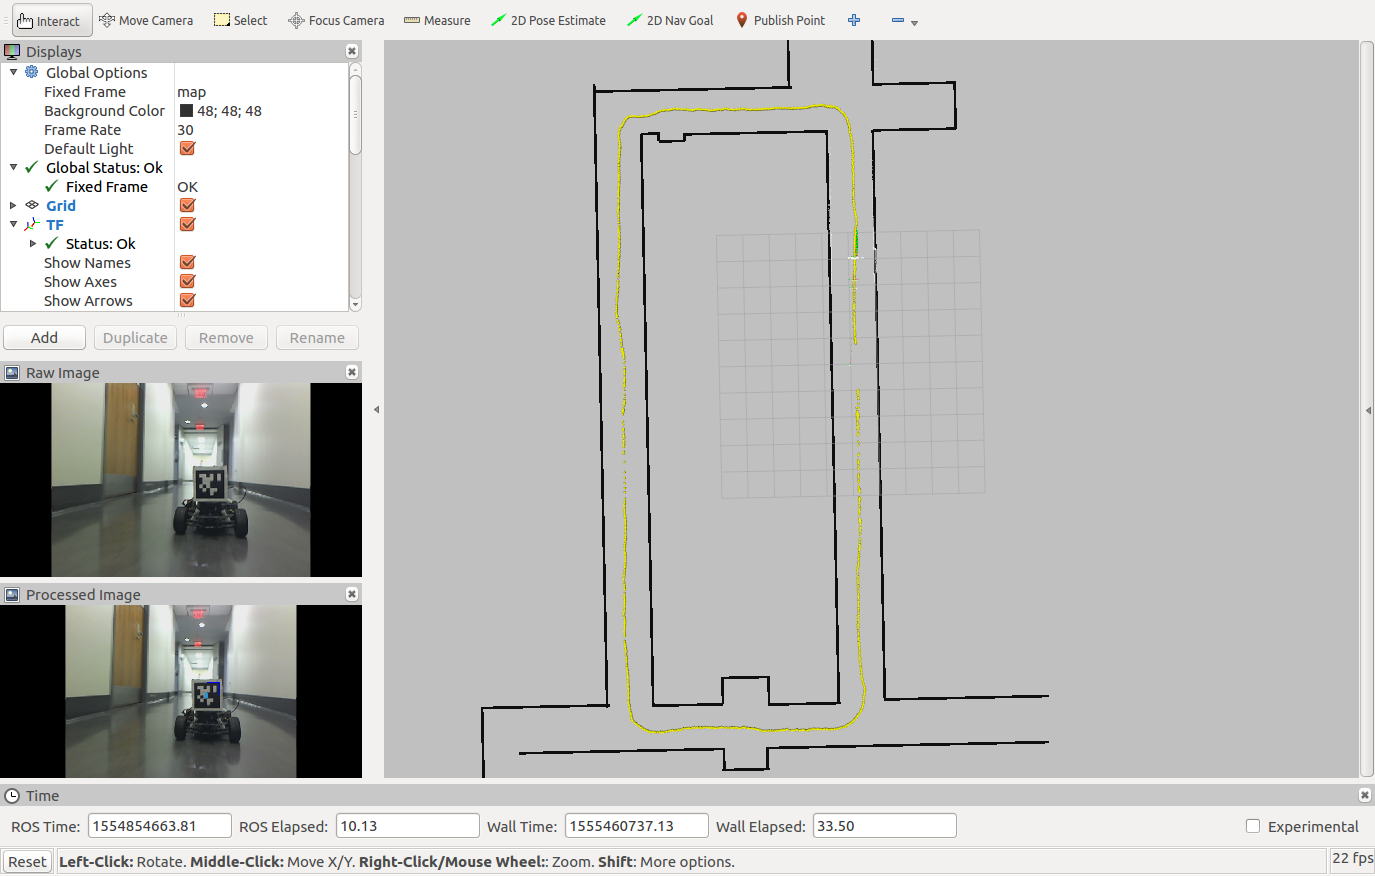
\includegraphics[width=0.5\textwidth]{waypoints.png}
   \caption{Predicting Poses over Rviz}
\end{figure}


\subsection{Deliverables}
You should submit the following items: a video of your detection and prediction pipeline. A plot showing the mean and variance of the detected poses publishing frequency. 

\section{Extra Credit}
You may already be doing some of these things for your project, this is some encouragement to get started early. The mechanical design and TX2 kernel support tasks have slightly flexible deadlines, see your TAs. The other tasks must be submitted with your lab to receive the bonus points. Extra credit will be awarded on an individual basis. If multiple team members participate you must use git to track contributions and supply the teaching staff with relevant commit history and a summary of who did what. The teaching staff's decisions about partially completed tasks and sufficiency of contributions by an individual working in a team are final. 

\subsection{Mechanical Design} \textit{\textbf{(10 pts added to lowest lab score)}}

\noindent Create a 3D printed mount for the realsense or logitech cameras
\newline

\noindent\textit{\textbf{(10 pts added to lowest lab score)}}

\noindent Create a mount for placing an AprilTag on the back of the car (3D printed and laser cut)
\newline

\noindent\textit{\textbf{(10 pts added to lowest lab score)}}

\noindent Fabricate the designs for the rest of the class once submitted (you need certification from MEAM to use these tools). 

\subsection{Improved Prediction} \textit{\textbf{(5 pts added to lowest lab score)}}

\noindent Use RRT, RRT$^{*}$, or follow-the-gap instead of pure-pursuit within the prediction algorithm. Can you weight the predictions from multiple algorithms? How would you decide the weighting etc. 
\newline

\noindent\textit{\textbf{(10 pts added to lowest lab score)}}

\noindent Use MPCC within the prediction algorithm. 

\subsection{Update the TX2 Kernel to support RealSense Camera} \textit{\textbf{(5 pts added to lowest lab score)}}

\noindent Provide a script and verify with the TAs so we can distribute this to the rest of the class. Be careful, hacking without understanding can brick your TX2. 

\subsection{YOLO pipeline}\textit{\textbf{(10 pts added to lowest lab score)}}

\noindent Replace the AprilTags pipeline with YOLO keep output of detected poses the same etc. 

\end{document} 
